\section{Profiling the \acs{MPM} and \acs{NLP}}
Producing $\bthstar$ via generation of the initial guess using the \ac{MPM},
and subjecting this to numerical optimisation involves operations which can be
computationally demanding, both in terms of the amount of work done by the
\ac{CPU}, and space requirements (i.e. the amount of \ac{RAM} required to store
all the required information as the routine runs). For the \ac{MPM}, the most
demanding aspect is \ac{SVD} calculations, which for numerical optimisation, it
is generation of the Hessian matrix. Detailed accounts of the computational
complexity of the \ac{MPM} and \ac{MMEMPM} has been described previously.
However, it is useful to consider what the actual running times of these
routines are. This is particularly useful, as a lot of the accounts on running
the \ac{MPM} are from decades before this work, and so the speed at which the
estimation routine can be expected to take will have decreased a lot thanks to
improvements in processing power. As an example, the account by Pines a
coworkers from 1997 states that a signal with $\None = 1024$ would take about
\qty{4.5}{\minute} to be processed by the \ac{MDL} and \ac{MPM}, using a
\qty{100}{\mega\hertz} \ac{CPU}\cite{Lin1997}. On the system used for all
results generated for this work (see Remark \ref{rem:workstation}), an
equivalent computation takes about \qty{100}{\milli\second}.
\begin{remark}
    \label{rem:workstation}
    All results generated in this work were acquired using a workstation
    featuring a Intel\textregistered\ Core\texttrademark\ i9-10900X CPU @
    \qty{3.7}{\giga\hertz}, and \qty{32}{\gibi\byte} of RAM.
\end{remark}

To gain a more concrete understanding
of\note{...}

\begin{figure}
    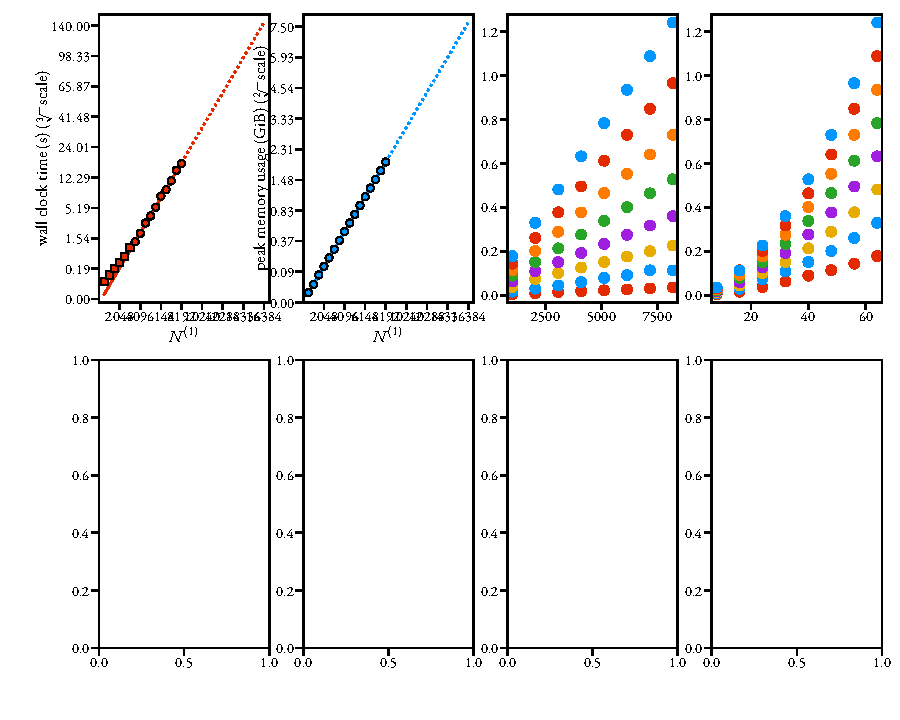
\includegraphics{timings/timings.pdf}
    \caption{TODO}
    \label{fig:profiling}
\end{figure}

\note{
\begin{itemize}
    \item 1D MPM: created signal with 10 oscs, varied $\None$ from  $512 \rightarrow 8192$ in steps of 512. $\Lone = \None / 3$
    \item Total time very closely agreed with tiem to compute SVD of  $\HY$, especially for larger  $\None$: cubic dependence found.
    \item Panel a in plot:  $\None$ vs wall clock time, with cube root scale.
    \item Linear fit to circular points is shown (for square points (small
        $\None$), other parts of the algorithm (notably EVD of VM1+VM2) had an
        appreciable impact on time.
    \item Peak memory requirement showed perfect quadratic relationship. Why?
    \item Extrapolated linear fit shows that unless very big signals
        considered, modern PCs should be able to cope.
\end{itemize}
}
